\documentclass[12pt,letterpaper]{article}
\usepackage[utf8]{inputenc}
\usepackage{natbib}
\usepackage{graphicx}
\usepackage{indentfirst}
\usepackage{indentfirst}
\usepackage[left=3cm,right=2cm,top=2cm,bottom=3cm]{geometry}

\usepackage{lipsum}

\setlength{\parindent}{2cm}
\setlength{\parskip}{\baselineskip}
\renewcommand{\baselinestretch}{1.5}

\renewcommand\contentsname{Índice de contenidos}
\renewcommand\refname{Referencias}

\begin{document}

\newpage
\vspace*{-.5cm}
\begin{picture}(18,4)(0,40)
	\put(350,-20){
\includegraphics[scale=.25]{images/LogoUsach.pdf}}
\end{picture}

\sloppy
\thispagestyle{empty}
\vspace*{-1.6cm}

\begin{center}
	{\bf \mbox{\large UNIVERSIDAD DE SANTIAGO DE CHILE}}\\
	{\bf \mbox{FACULTAD DE INGENIER\'IA}}\\
	{\bf \mbox{DEPARTAMENTO DE INGENIER\'IA INFORM\'ATICA}}\\
\end{center}

	\vspace*{3cm}
	\par
	\vspace{1cm}
	\begin{center}
	\large
		Organización de Computadores\\Laboratorio \#1
	\end{center}
	\vspace{3cm}
	\begin{flushright}
		\begin{tabular}[t]{l l}
			Integrantes: & Nestor Mora \\
			             & Cristian Espinoza \\
			Profesor(a): & Nicolas Hidalgo \\
						 & Erika Rosas \\
			Ayudante: & Felipe Fuentes\\

		\end{tabular}
	\end{flushright}
	\begin{center}
		\vspace{3cm}
		Lunes, 6 de Octubre de 2014
	\end{center}



\newpage
\tableofcontents
\thispagestyle{empty}

\newpage
\renewcommand{\thepage}{\arabic{page}}
\setcounter{page}{1}
\section{Introducción}
El presente informe, detalla elaboración del Laboratorio 1 del ramo Organización de Computadores, el cual consiste en la producción de una aplicación que desarrolle el logaritmo natural de un número, pero resuelto a través del uso de la Serie de Taylor.

El objetivo principal es disminuir el tiempo de ejecución de la aplicación.

Los objetivos específicos son la elaboración de la aplicación que desarrolle la serie de Taylor para resolver el logaritmo natural de un número, detectar los hazards y la disminución en la cantidad de tareas realizadas en el proceso de calcular la serie.

Para disminuir el tiempo de ejecución de la aplicación, se ha procedido a considerar los hazards y a través del uso de pipeline, reordenar algunas instrucciones para que no exista la necesidad de esperar los resultados.
\newpage
\section{Marco Teórico}
\subsection{Serie de Taylor}
La Serie de Taylor es una serie funcional y surge de una ecuación en la cual se puede encontrar una solución aproximada a una función.

Ésta sirve para conseguir una aproximación del valor de una función en un punto.

\subsection{Pipeline}
Es una técnica de implementación en la cual múltiples instrucciones están traslapadas en la ejecución. Esto sirve para disminuir el tiempo de ejecución de un programa.

\subsection{Getopt}
Es una biblioteca de funciónes C, utilizado para analizar las opciones de línea de comandos .
También es el nombre de un programa de Unix para analizar los argumentos de línea de comandos en shell scripts.%agregar referencia http://en.wikipedia.org/wiki/Getopt
\newpage
\section{Desarrollo}
\subsection{Gráfico de iteraciones}
\begin{picture}(100,175)(0,40)
	\put(-50,5){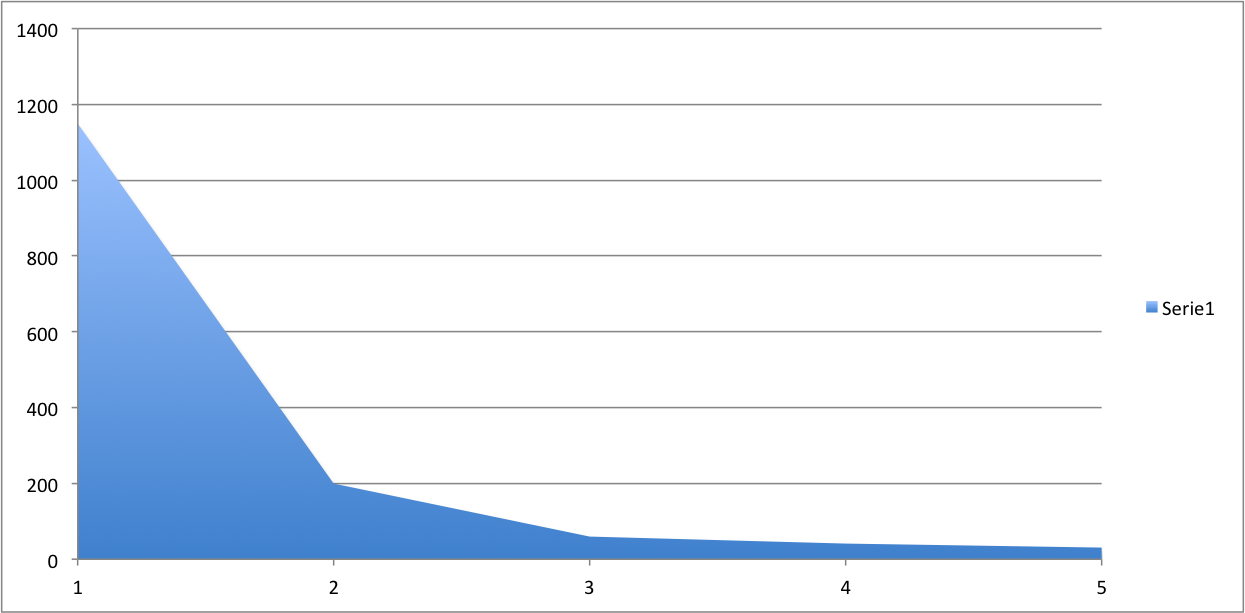
\includegraphics[scale=.75]{images/graf1.png}}
\end{picture}
\subsection{Descripción del problema}
Se pide realizar la Serie de Taylor para resolver el logaritmo natural de un número, para luego ir mejorando el código, y después de eso, a través del uso de pipeline ir disminuyendo el tiempo de ejecución de este.

\subsection{Primer Paso - main0.c}
Lo primero que se realizó, fue escribir el programa tal cual se presentó en el ejemplo, ésto es definiendo el valor de las constantes que se encuentran en el desarrollo de la serie de taylor, realizando la fracción en la función de logaritmo natural, para luego realizar las multiplicaciones de estas fracciones con las constantes.

\subsection{Segundo Paso - main1.c}
Lo segundo en hacer fue colocar el desarrollo de la fracción en la parte principal del programa, para así no calcularlo en cada multiplicación de la función logaritmo, sino que solo multiplicar el resultado ya obtenido para así calcular la serie de taylor, dentro de este mismo paso, se decidió aumentar la cantidad de constantes y por lo tanto la cantidad de multiplicaciones realizadas al calcular la serie de taylor, ésto para que el valor obtenido sea más cercano al valor real del logaritmo natural, aquí se presenta la primera gran problemática, ya que al aumentar demasiado la cantidad de constantes, el programa demora más tiempo al calcular el valor, así que se decide trabajar solo con 20 constantes.

\subsection{Tercer Paso - main2.c}
Se decide trabajar con los valores ya calculados, es decir, ir agregando a la multiplicación ya realizada, el valor que debe ser multiplicado después, disminuyendo así la cantidad de multiplicaciones que deben realizarse.

\subsection{Cuarto Paso - main3.c}
Del programa anterior, se decidió que en la linea "retorno += c2 * x\_2nplus1;" se están realizando 2 operaciones, una multiplicación y una suma, ademas de tener dependencia de la linea anterior "x\_2nplus1 *= x\_cuad;", considerando esto se decidió aumentar en una linea, y en ella depositar en una variable temporal "temp=c2 * x\_2nplus1;" con ello se manejan las dependencias, reduciendo el tiempo de ejecución.


\subsection{Quinto Paso - main4.c}
En el quinto paso se decidió cambiar la función que va ocupando los valores ya calculados, por una función que es netamente la factorización de lo que realiza la multiplicación en la serie de taylor, ya teniendo calculados dos valores que se repetirán a lo largo de la función que son x al cuadrado y x a la cuarta.
\newpage
\section{Discusiones}
Al momento de crear el primer programa (main0), los resultados el tiempo era bastante alto, ésto se debía a que el programa en la obtención de cada término de la serie de taylor, realizaba la fracción que se necesitaba para obtenerlos, ya que el programa realizaba ésta tarea, obtuvimos que se demoraba 1150 ns/call, lo cual es bastante para un programa que solo calcula la serie de taylor.

Para mejorar ésto se realizó el segundo programa (main1) donde la realización de estas fracciones se hacía en la parte inicial del programa, haciendo así que el programa disminuyera su tiempo de forma considerable, ya que el valor de la fracción se calcula solo una vez, además, se nota que existe hazard en la obtención del valor x y el calculo de la fracción, separándolo entonces, en 3 funciones diferentes que pudieran éstar lo suficientemente distantes para no tener que esperar el valor de alguna para calcular el de la siguiente, por eso, encontramos que se calculan los valores de numerador y denominador, y luego se establecen otros valores, para luego calcular el valor de la fracción, así, no es necesario "esperar" los valores de numerador y denominador, ya que se encuentran calculados para este punto, gracias a esto se obtenie una mejora en el tiempo de ejución, bajando a 200,43 ns/call.

Con estos datos aun no se lograba el resultado esperado, así que fue necesario implementar otra forma de realizar la serie de taylor, ésto fue multiplicando los datos anteriormente calculados, disminuyendo también la cantidad de multiplicaciones, puesto que ya no debia calcularse los valores a cada momento, sino ir aumentando el valor; así es como se obtiene una mejora bajando a 60,21 ns/call.

El cambio siguiente fue más que nada en los hazards ya que habían tiempos en que se necesitaba esperar los valores de multiplicaciones anteriores, es así como se mejora ésto con el uso de un temporal donde se almacena un dato y con esto se manejan las dependencias y se disminuye el tiempo de ejecución a 40,13 ns/call.

Si bien se logra disminuir el tiempo de ejecución utilizando los valores multiplicados anteriormente y aumentándolos, se intenta con una factorización de los valores a multiplicar, con ésto se disminuye aun más el tiempo de ejecución del programa, si bien se logran ver algunos hazards, no encontramos formas de disminuirlos con la última forma elegida; pese a esto, se decide dejarla como la función final, ya que aun con los hazards, éste programa demora menos tiempo, quedando así en 30,13 ns/call.

\newpage
\section{Conclusión}
Frente a la problemática de crear el programa, éste fue confuso al inicio ya que al inicio fue complicado entender la actividad a realizar, además del poco conocimiento en github, hazards y pipeline. Una vez entendido todo esto fue menos complejo el poder avanzar en el trabajo realizado.

Se logró cumplir con los objetivos del trabajo, tanto el objetivo principal como los objetivos específicos, disminuyendo el tiempo de ejecución del programa; aunque creemos que éste puede reducirse más, nos vemos limitados a nuestros conocimientos actuales y a nuestra poca experiencia frente al tema, ya que, nosotros creemos que ya se encuentra bastante reducido el tiempo de ejecución y no se nos ocurren otras formas de reducirlo más.

Además, el programa funciona correctamente y logra obtener el resultado esperado en mucho menor tiempo que el primer programa realizado.

\newpage
\addcontentsline{toc}{section}{Referencias}
\bibliographystyle{plain}
\bibliography{references}

\end{document}
